\documentclass[tikz]{standalone}
\usepackage{amsmath}
\begin{document}
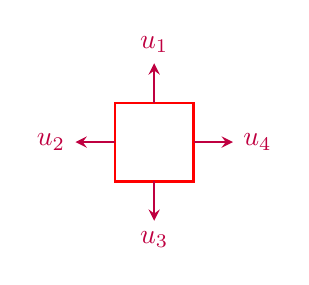
\begin{tikzpicture}[>=stealth,thick]

  % 正方形:边长 1, 中心在原点(顶点为 (-0.5,-0.5) 到 (0.5,0.5))
  \draw[red] (-0.5,-0.5) rectangle (0.5,0.5);

  % 四个方向的箭头与标签
  % 上:u_1
  \draw[purple,->] (0,0.5) -- (0,1.0) node[above] {$u_{1}$};
  % 下:u_3
  \draw[purple,->] (0,-0.5) -- (0,-1.0) node[below] {$u_{3}$};
  % 左:u_2
  \draw[purple,->] (-0.5,0) -- (-1.0,0) node[left] {$u_{2}$};
  % 右:u_4
  \draw[purple,->] (0.5,0) -- (1.0,0) node[right] {$u_{4}$};

  % 辅助坐标轴(可选):如不需要可删除以下两行
  % \draw[->,gray] (-1.2,0) -- (1.2,0) node[right] {$x$};
  % \draw[->,gray] (0,-1.2) -- (0,1.2) node[above] {$y$};

\end{tikzpicture}
\end{document}
